\documentclass[scheme=plain,12pt]{ctexart}

\usepackage{graphicx}
\usepackage[hmargin=1.1in,vmargin=1in]{geometry}
\usepackage{indentfirst}

\fontsize{14pt}{1.0}

\newlength{\blanklength}
\setlength{\blanklength}{40ex}

\providecommand{\thetitle}{信号处理与电生理学技术}
\providecommand{\theauthor}{Sparky\_14145}
\providecommand{\thestudentID}{71XXXXXX}
\providecommand{\theemail}{Sparky\_14145@outlook.com}
\providecommand{\theinstitution}{软件工程学院}

\input{personal_info/info.tex}

\providecommand{\blankToFill}[1]{
    \parbox[t][3ex]{\blanklength}{
        \makebox[\blanklength]{#1}\\[0pt]
        \rule[2ex]{\blanklength}{0.1ex}
    }
}

\providecommand{\makecover}{\begin{titlepage}
    \noindent
    {Course Report} \\[2pt]
    {\large \bfseries Southeast University}

    \vspace*{20pt}
    \begin{center}
    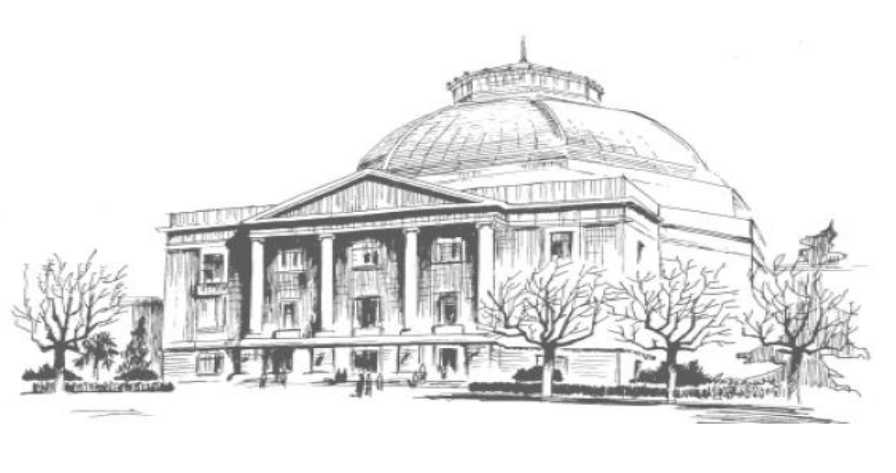
\includegraphics[width=0.9\textwidth]{pics/cover.png}\\
        \textsc{\Huge 信号处理导论}

        \vspace*{10pt}
        \begin{tabular}[c]{rc}
            题目        & \blankToFill{\thetitle} \\
            日期        & \blankToFill{\today} \\
            作者        & \blankToFill{\theauthor} \\
            学号        & \blankToFill{\thestudentID} \\
            学院        & \blankToFill{\theinstitution}
        \end{tabular}
        \rmfamily
    \end{center}

    % \vspace*{0pt}
    % \begin{abstract}
    %     Advanced data structures are the data structures that have advanced features,
    %     like staying effective without using extra storage space (\emph{Splay trees}),
    %     holding persistent data while having short access and modify time (\emph{Persistent
    %     Segment trees}) or easy to implement but fast to use in most situations (\emph{Skip
    %     lists}). Advanced data structures are invented to solve different problems that
    %     the data structures before cannot solve, so there is no ``universal'' ways to
    %     make a data structure ``advanced''. but there are still some common thoughts in parts
    %     of these structures, like their ways to hold persistent data and their ways to reduce
    %     complexity of operations. Like all other things, the advanced data structures are
    %     under continous development. The trends of advanced data structures are: they are
    %     going to be more and more complex (both in relationships between data and in algorithms
    %     to access and maintain the structures), they are more and more running on distributed
    %     systems and decentralized environments.
    % \end{abstract}
    % \footnotetext{\theemail}

    \tableofcontents
\end{titlepage}}

\begin{document}
    \makecover

    \section{信号}

    信号是一种信息流,是``传递有关一些现象的行为或属性的信息的函数''。在现实世界中,任何随时间或者空间变化的量(如影像)
    都是潜在的信号,它们可能会提供一个物理系统的状态信息,或在不同观察者之间传达消息等。《IEEE信号处理汇刊》阐述“信号”一
    词如下:

    \begin{quote}
        术语“信号”包括音频、视频、语音、图像、通信、地球物理、声纳、雷达、医疗和音乐信号等。
    \end{quote}

    自然地,生物体内的不同部位的电势差或者电流也能够``传达消息'',因此也是一种信号。

    \section{电生理学}

    电生理学是生理学的一个分支,是一门研究生物细胞或组织的电学特性的科学,主要研究神经元的电学特性,尤其是动作电位包括
    细胞膜电势变化与跨膜电流的调节。它涉及在多种尺度上从单个离子通道蛋白到整个器官如心脏的电压变化或电流变化的测量值。在
    神经科学,它包括神经元的放电活动的测量,特别是动作电位的活动。记录来自神经系统的大规模电信号,如脑电图的记录,也可以
    被称为电生理记录。

    \subsection{经典电生理学}

    经典电生理学通过各种测定、记录电信号的方法,来测量神经元的离子变化,进而推断神经元的生理状态。最为典型的测定技术是插入
    电极。典型的电极有如下种类:

    \begin{itemize}
        \item 简单电极,比如说电极片,电极针或者电极针阵列;
        \item 集成电路板或其他可折叠的介质;
        \item 空的外壳包裹的电解质。
    \end{itemize}

    通过检测神经元的电信号变化,神经科学家可以检测个体的脑部活动,进而确定神经紊乱是怎么发生的。如果电极足够小,那么它
    就可以被刺入单个神经元细胞,并准确地检测这个细胞的电活动。但是这种侵入式方法容易降低神经元细胞的寿命,并对个体的神经
    系统造成不利影响。其他的记录方式包括膜片钳技术等。

    \subsection{光电生理学}

    经典电生理学方法的观察与记录通常只针对某一个或几个特定的神经元细胞,如果需要从宏观上了解神经活动,就需要用到光电生理
    学方法。光电生理学通过利用某些分子能够在特定电或化学环境下发出光的特性,将诸如光敏颜料等物质导入神经元或覆盖在神经元
    上,进而将神经活动的电信号转化为光信号以方便研究。

    \section{膜片钳技术}

    膜片钳技术是一种电生理学实验技术,用于研究组织切片、单个分离细胞或一小块细胞膜的离子电流。这项技术可应用于研究可兴奋
    细胞,比如神经元、心肌细胞、肌细胞和胰岛β细胞,也可以应用于细菌特别是制备的大型原生质球上的离子通道研究。

    膜片钳技术可以有电压钳和电流钳两种设置,在电压钳中,设备通过负反馈电路维持细胞跨膜电位在某一数值来观察跨膜电流的变化,
    而在电流钳中,微电极向细胞内注入恒定或变化的电流,记录相应膜电位的变化,如动作电位的形成。

    膜片钳技术的基本思路是利用一个与神经元直接接触(但不刺穿细胞膜)的记录电极,和一个浸泡在浴液中的参比电极,将神经元细
    胞和浴液置入一个回路,并记录回路两端的电压变化(电压钳设置)或是在特定电压下回路中电流的变化(电流钳设置)来追踪神经
    元的动作。

    电压钳设置下,需要用到一个差分放大器来记录记录电极和参比电极之间的电势差。并且在一部分实验中,玻璃管需要在拉针仪中加
    热以产生光滑的尖头表面,使其和细胞膜的密封性更好,从而有更高的电阻,进而减少其他电流的产生,在提高记录的机械稳定性同
    时降低电信号噪声。

    膜片钳技术有几种不同的基本记录模式,包括细胞贴附式、内面向外式、全细胞记录式、外面向外式、穿孔膜记录式和松散封接是。
    这些记录模式有各自的特点,采用的记录电极也不尽相同,具体采用哪种则取决于研究人员想要得到哪些数据。

    另外有一种较新的,称为``全自动膜片钳''的技术,可以在较短的时间内以低廉的价格获取大量数据。

    \section{脑电图、颅内脑电图}

    脑电图是一种记录脑电波的电生理监测方法,常用于诊断癫痫等,是一种比较传统和常见的脑部研究手段和脑部疾病诊断方法。它
    利用在头皮放置一定量的电极,具有便捷、无创伤等优势,但是容易受到环境等其他因素干扰,因此往往需要结合其他的手段来确
    定具体的病症。

    尽管现在有核磁共振、电脑断层扫描等各种高分辨率解剖成像技术,但是脑电图能够提供精确至毫秒的时间分辨率,故脑电图仍然
    是脑研究与诊断的宝贵工具。

    颅内脑电图则是一种侵入式的电生理监测方法,通过开颅手术等方法将电极直接放置在大脑皮层裸露表面上,来记录大脑皮层的神
    经活动,因为相对不易受到各种环境干扰而拥有比(颅外)脑电图更高的准确性。但颅内脑电图也存在着一些局限,比如说麻醉会
    影响记录结果,采样时间受限(导致部分病症可能不会被记录),以及观测范围有限(可能导致取样错误)。

    \section{皮层刺激测绘}

    皮层刺激测绘是一种包含物理侵入式过程的电生理学手段,其目标是将脑的各个区域与其功能建立联系。皮层刺激测绘将电极置入
    到硬脑膜下,但与颅内脑电图不同的是,皮层刺激测绘的电极会主动向其所植入的区域施加电流,对其造成刺激甚至是可逆的损伤,
    然后观测目标区域的神经元和受试者的反应与行为变化,进而推断目标区域的功能及其是否存在异常。

    刺激电流大小是皮层刺激测绘中至关重要的一个项目。一般来说,如果控制得当,受试者在接受完皮层刺激测绘以后,受试区域不
    会受到损伤。具体操作时,往往需要反复调节刺激电流,从一个较低的电流开始,每次逐渐增加电流的强度,直到受试者出现
    反应(如肌肉动作等)后停止。

    皮层刺激测绘往往和颅内脑电图同时使用。

\end{document}